% ****** Start of file apssamp.tex ******
%
%   This file is part of the APS files in the REVTeX 4 distribution.
%   Version 4.0 of REVTeX, August 2001
%
%   Copyright (c) 2001 The American Physical Society.
%
%   See the REVTeX 4 README file for restrictions and more information.
%
% TeX'ing this file requires that you have AMS-LaTeX 2.0 installed
% as well as the rest of the prerequisites for REVTeX 4.0
%
% See the REVTeX 4 README file
% It also requires running BibTeX. The commands are as follows:
%
%  1)  latex apssamp.tex
%  2)  bibtex apssamp
%  3)  latex apssamp.tex
%  4)  latex apssamp.tex
%
\documentclass[twocolumn,showpacs,preprintnumbers,amsmath,amssymb]{revtex4}
%\documentclass[preprint,showpacs,preprintnumbers,amsmath,amssymb]{revtex4}

% Some other (several out of many) possibilities
%\documentclass[preprint,aps]{revtex4}
%\documentclass[preprint,aps,draft]{revtex4}
%\documentclass[prb]{revtex4}% Physical Review B

\usepackage{graphicx}% Include figure files
\usepackage{dcolumn}% Align table columns on decimal point
\usepackage{bm}% bold math

\graphicspath{{../figures/}}

%\nofiles

\begin{document}

\preprint{APS/123-QED}

\title{Characterizing the Efficiency-Robustness Trade-offs in US Domestic Airline Networks}% Force line breaks with \\

%\author{Ann  Author}
% \altaffiliation[Also at ]{Physics Department, XYZ University.}%Lines break automatically or can be forced with \\
%\author{Second Author}%
% \email{Second.Author@institution.edu}
%\affiliation{%
%Authors' institution and/or address
%}%
%
%\author{Charlie Author}
% \homepage{http://www.Second.institution.edu/~Charlie.Author}
%\affiliation{
%Second institution and/or address% with \\
%}%

\date{\today}% It is always \today, today,
             %  but any date may be explicitly specified

%\begin{abstract}
%We present a study of efficiency and robustness of several real world complex networks. We report a detailed analysis of the topologies of major US domestic airlines networks. We also analyze other classes of complex networks, such as food-webs, trade networks and supply-chains. Interesting structural motifs can be observed both within and across classes of networks. Some of these motifs are potential design principles for complex networks.
%\end{abstract}

\pacs{Valid PACS appear here}% PACS, the Physics and Astronomy
                             % Classification Scheme.
%\keywords{Suggested keywords}%Use showkeys class option if keyword
                              %display desired
\maketitle

\section{\label{sec:intro}Introduction}

Airline networks form the backbone that carries the bulk of a country's transportation load. The US domestic airlines carried more than 53 million people in the first quarter of 2009, over 746,400 flights, amounting to a revenue of more than 46 billions~\cite{stats2009}. In addition to catering to transportation needs, airline networks have long reaching socio-political impacts. They are critical infrastructure wherein operational inefficiencies can cost billions of dollars every year~\cite{button99, brueckner05, morrison07}. In recent times, airline networks also pose the threat of propagating contagious diseases such as SARS and swine influenza~\cite{colizza06}. 

Airline networks have evolved over a period of time as a result of design decisions governed largely by economic considerations of airline companies, and constrained by geo-political relations between countries~\cite{guimera05}. There are studies on the impact of the hub and spoke structure of US domestic airlines following deregulations in the 1970s. There are conflicting views on the economic advantages of hub and spoke structures as opposed to point to point structures~\cite{brueckner01, burghouwt02, button02, berry06}. Recently, there are suggestions that a co-existence of hub and spoke and point to point networks can lead to stable equilibria by means of game theoretic analyses~\cite{alderighi07}.

The underlying structure or topology of an airline network not only impacts its day to day performance, but also its resilience in the phase of uncertainties and disasters. The structure also influences important decisions such as location of hubs, airline code sharing, mergers~\cite{adler06, alumur08}, schedules and pricing~\cite{berry06, mcafee06, forbes08}. Hence, a detailed understanding of the structure of airline networks is important.

In this work, we analyze the networks of seven major US domestic carriers from a complex networks perspective. We study their structural properties with respect to two parameters critical to network performance: \textit{efficiency} and \textit{robustness}. We characterize the trade-offs between efficiency and robustness in terms of multiple performance metrics using a graph theoretic framework. We observe that US domestic airline networks have similar structural properties that are possibly a result of similar design trade-offs.%[SANKET: Need to come back to this based on results.]

%[SANKET: Refine the following paragraphs.]
There are several efforts in the last few years towards analyzing airline networks. Guimer\`{a} \textit{et al.}~\cite{guimera04} study the world-wide airport network (WAN) and report ``anomalous'' high betweenness centrality values for nodes that have relatively low degrees. They argue that power-law generating models such as \textit{preferential attachment} (PA) cannot explain this observation. Instead, they propose that the anomalous centrality is a result of a network designed under several geo-political constraints leading to well-defined, geographically separated community structures~\cite{guimera05}. Further, they classify cities based on their intra and inter-community ``participation'' into roles such as hubs, provincial hubs, connectors and peripheral nodes.

Barrat \textit{et al}.~\cite{barrat04} consider a weighted network model of WAN, and analyze the degree and betweenness distributions, clustering coefficient and the \textit{mixing pattern}~\cite{newman03} of nodes. Here, weights on edges are expressed in terms of the number of available passenger seats between pairs of airports. They report that considering weights allows a richer characterization of a network. In a related work, Barth\'{e}lemy \textit{et al}. propose a model of network evolution based not only on the network topology, but also on the strengths of interaction between nodes represented by edge weights~\cite{barthelemy04}.

Colizza \textit{et al.}~\cite{colizza06} study the role of the air transportation network in the spreading pattern of diseases. They report a correlation between the heterogeneity in the structure of the air transportation network and the seemingly erratic, global scale sprading of diseases.

Domestic airline networks have also been studied in an effort to better understand the dynamics of transportation networks at a lower scale. Li and Cai~\cite{li04} observe that the degree distribution of the airport network of china (ANC) follows a double Pareto distribution. %They also define a simple measure of efficiency of the network. 
Bagler~\cite{bagler08} reports that the airport network of India (ANI) is a small world like ANC and WAN, however with a much smaller clustering coefficient. Further, ANI suggests a \textit{disassortative mixing} with hubs having a lot more low-degree neighbours than high-degree neighbours. This is in contrast with WAN wherein \textit{assortative mixing} can be observed~\cite{barrat04}. Similar analysis on the Italian airport network shows a small-world network characterized by a fractal nature~\cite{guida06}. Sienkiewicz and Ho\'{l}yst~\cite{sienkiewicz05} report a statistical analysis of transportation networks of 22 Polish cities. Similar to other networks in this class, small-world behaviour with a hierarchical structure is observed.

%[SANKET: Need to refine the following paragraphs.]
In general, the following approaches can be found in literature concerning the study of airline networks: (1) analyzing properties such as degree and node betweenness distributions, clustering coefficient and mixing, such that they can be related to standard network generation models like preferential attachment and small-world networks, and (2) developing a theory or model to generate networks that show properties characteristic of airline networks.
While these approaches have resulted in many important insights, there is still a need for an in depth understanding how different aspects of the structure of airline networks relate to their overall performance. Also, while network generation models explain certain properties, such as power law degree distributions or large clustering coefficients, there is a need to validate network generation models with respect to a wider set of properties~\cite{mitzenmacher}.

In this work, %we extend the formalism proposed by Venkatasubramanian \textit{et al}. to analyze the efficieny and robustness of
%US domestic airline networks. 
we use multiple metrics for efficiency and robustness that characterize the different aspects of optimality (or performance) in networks. We observe that the most of the seven airline networks that we study separately show similar trade-offs. %[NEED TO COMPLETE THIS.]
%[SANKET: Need some numbers and trends here.]
This work is part of a larger project in which we study several classes of real world complex networks including airline networks, food webs, supply chains and trade networks in search of structural motifs, within classes as well as across classes, that lead to optimal performance in disparate networks. We conjecture that these optimal motifs are potential underpinnings for designing new complex networks.

\section{Preliminaries}

\subsection{Data}

We consider seven major US domestic carriers: American Airlines, Southwest Airlines, Delta Airlines, United Airlines, Continental Airlines, US Airways and Northwest Airlines. Our data comes from the official flight schedules effective from May 1, 2008, available on the respective websites of the carriers. Table \ref{tab:eff} has information about the sizes of each airline network.

Every domestic airport served by a carrier is denoted by a node in the carrier's network. We do not consider international destinations. We also do not consider flights operated by subsidiaries. An edge in a carrier's network indicates the presence of at least one direct flight belonging to the carrier between a pair of nodes. We observe that all the networks are symmetric. That is, an edge exists in both directions between every pair of nodes in all the networks. Thus, we replace a pair of directed edges between nodes with a single bidirected or undirected edge. In the rest of the paper we consider all networks to be undirected.

%\begin{table*}
%\caption{\label{tab:table1}Summary of data for the seven domestic airline networks. The number of nodes, $n$, corresponds to the number of airports. An edge is present between two nodes in a network if there is at least one direct flight belonging to the carrier between the nodes. The three biggest hubs in each network are listed.}
%
%\begin{ruledtabular}
%\begin{tabular}{|c||c|c|c|c|c|c|c|}
% %&\multicolumn{2}{c}{$D_{4h}^1$}&\multicolumn{2}{c}{$D_{4h}^5$}\\
% Carrier & Southwest & American & Delta & United & Continental & US & Nortwest\\
% \hline
% \# Nodes ($n$) & 66 & 82 & 94 & 88 & 126 & 79 & 105\\
% \hline
% \# Edges ($e$)& 1742 & 207 & 210 & 205 & 269 & 207 & 207\\
% \hline
% \multirow {Major Hubs} & Las Vegas & Chicago & Cincinnati & Chicago & Cleveland & Charlotte & Detroit\\
% 	& Chicago & Dallas & Atlanta & Denver & Houston & Philadelphia & Memphis\\
%	& Phoenix & Lambert & New York & Los Angeles & Newark & Phoenix & Minneapolis
%\end{tabular}
%\end{ruledtabular}
%\end{table*}

Both unweighted and weighted networks are considered. Here, weights on edges are simply the distances between airports computed from latitude and longitude information using the haversine formula~\cite{haversine}.

\begin{figure*}
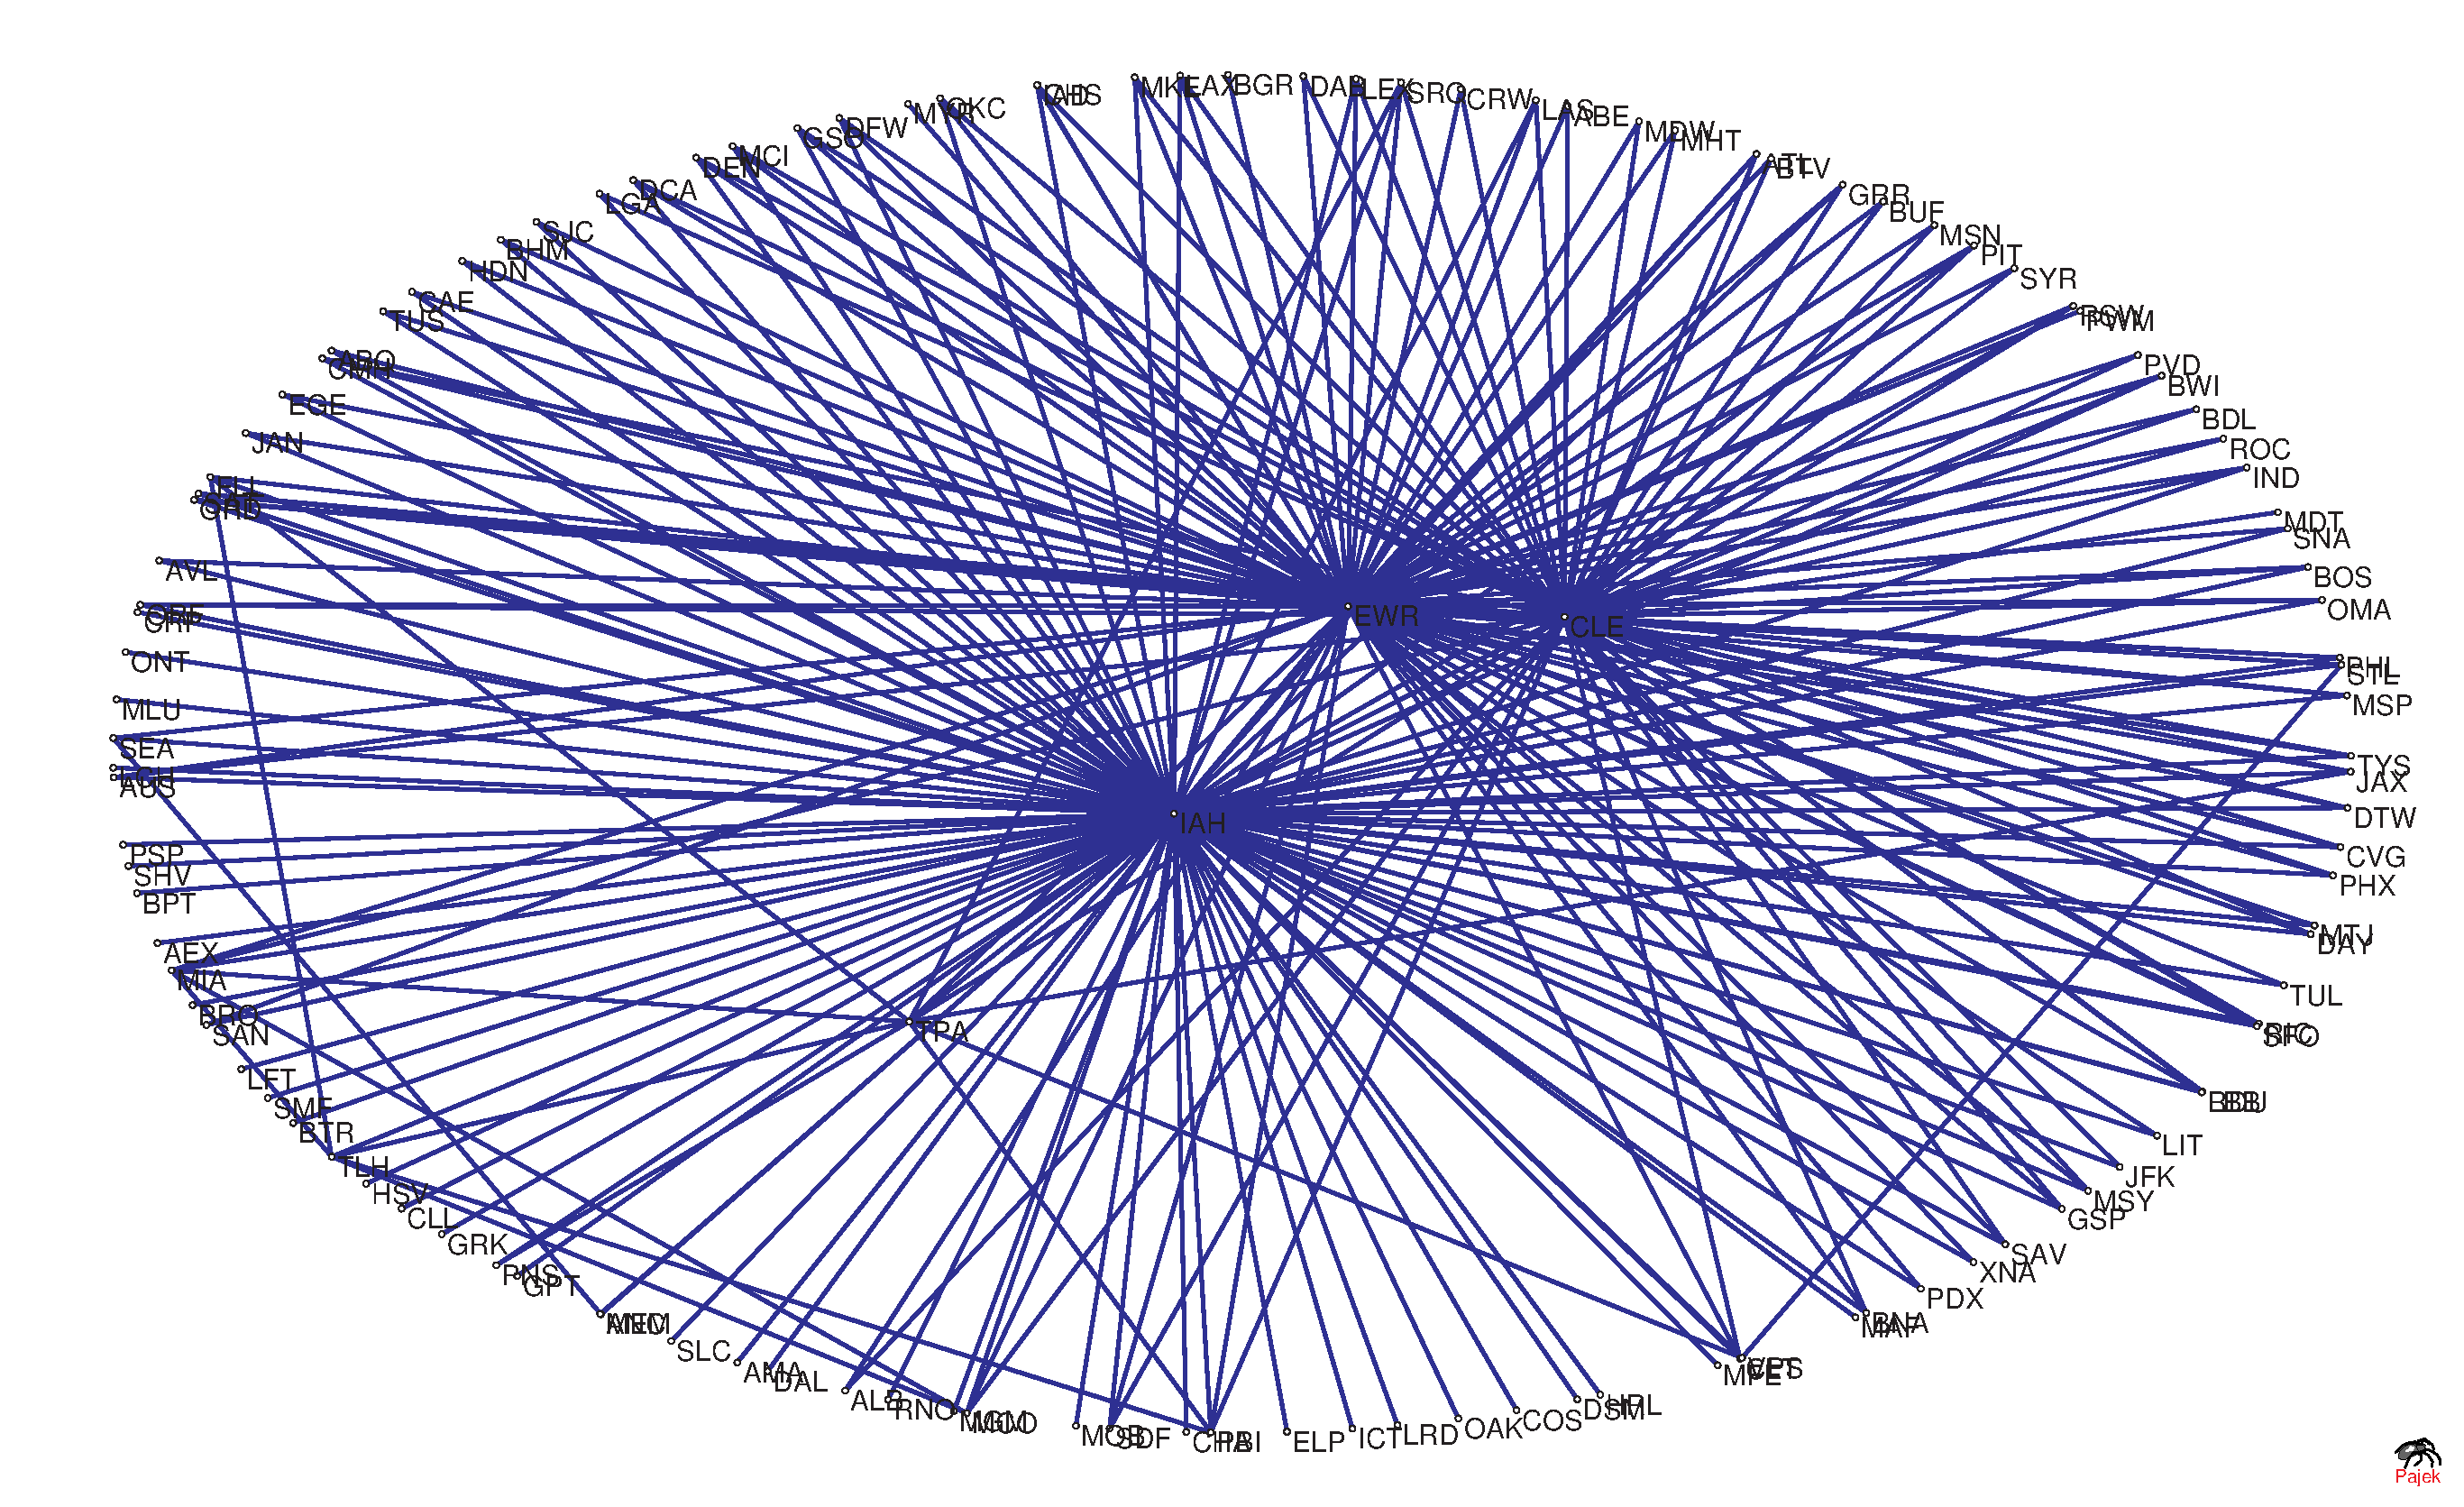
\includegraphics[width=7.5in]{continental-network}% Here is how to import EPS art
\caption{\label{fig:continental}Topology of Continental Airlines}
\end{figure*}

\begin{figure*}
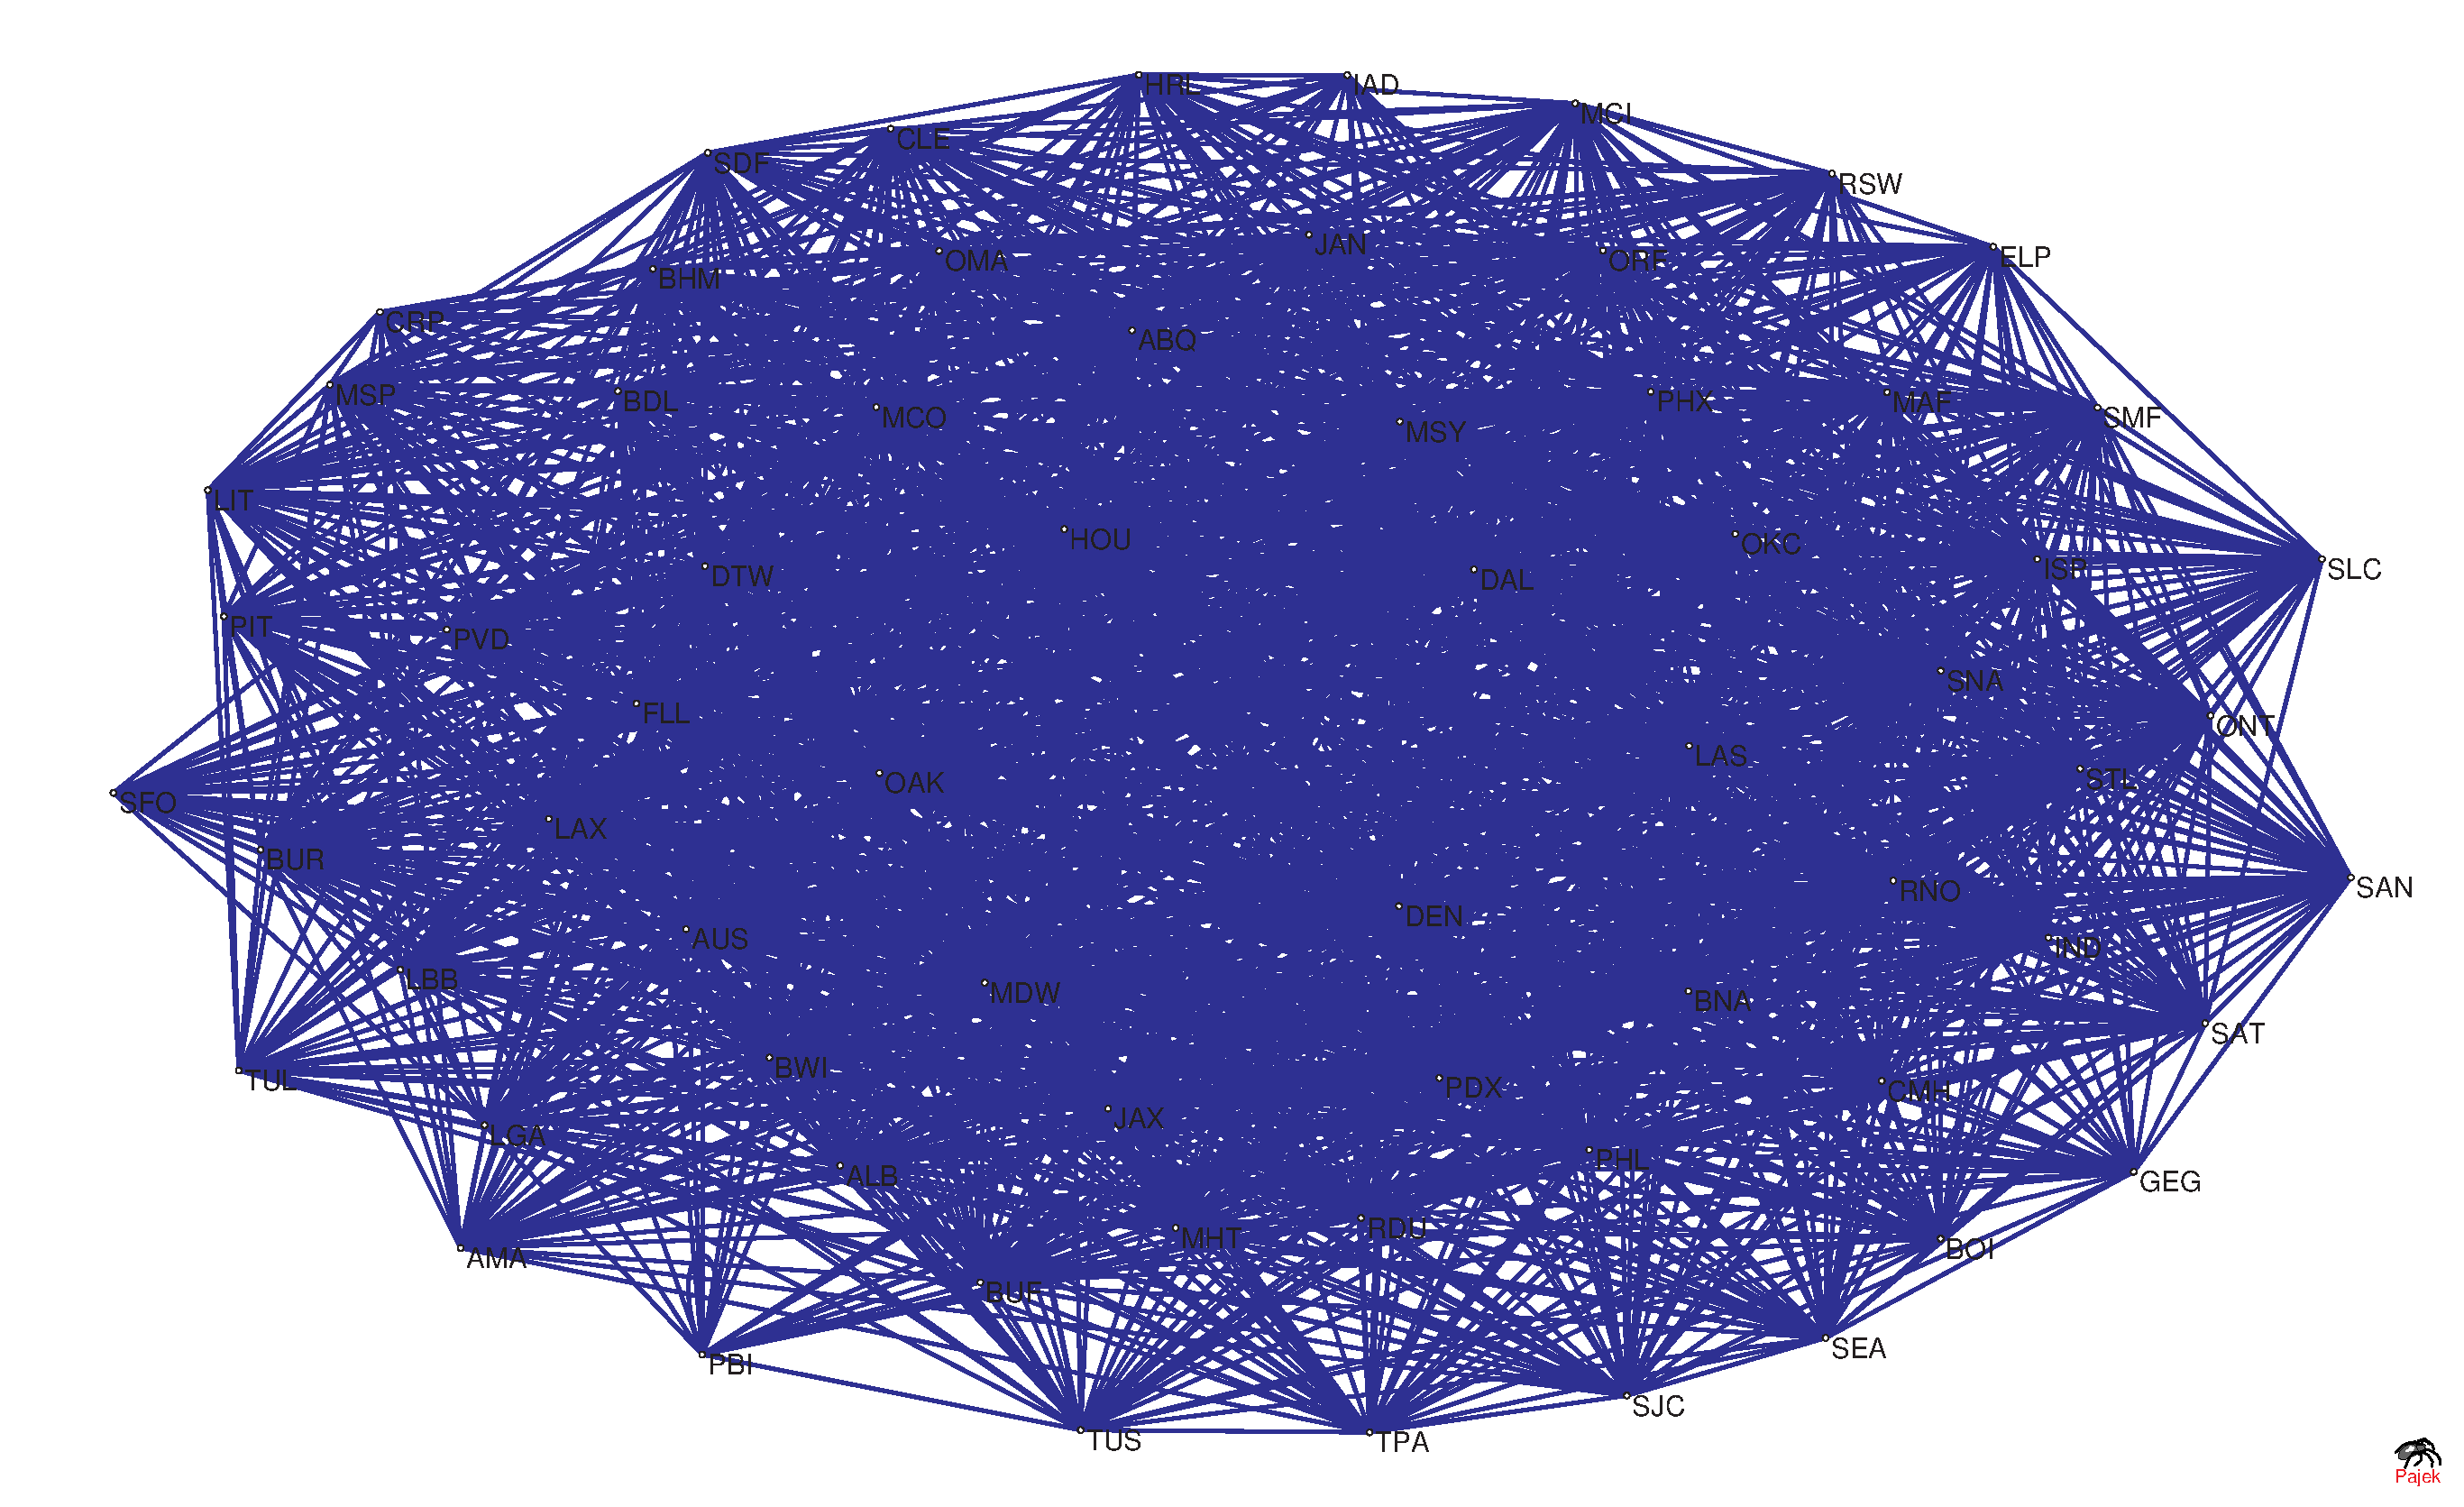
\includegraphics[width=7.5in]{southwest-network}% Here is how to import EPS art
\caption{\label{fig:southwest}Topology of Southwest Airlines}
\end{figure*}

\subsection{Network Analysis Framework}
Our framework is inspired by Venkatasubramanian \textit{et al.}'s~\cite{venkat04} work on the emergence of network topologies under varying constraints. %Venkatasubramanian \textit{et al}. propose that the structure of a network is a result of adaptation under trade-offs between three critical parameters: efficiency, robustness and cost. 
%Venkatasubramanian \textit{et al}.~\cite{venkat04}, study the emergence of network topologies under varying efficiency and robustness requirements. They propose a 
%[SANKET: Need to improve this.]
They propose a formalism based on the Darwinian evolutionary theory: networks evolve their structures so as to optimize their short term operational performance (efficiency) as well as long term survival chances (robustness). There is also a cost constraint that networks cannot breach. A selection pressure variable decides the trade-off between short term and long term survival goals. Efficiency is measured in terms of the average path length ($apl$) in the network. Robustness is measured in terms of the size of the largest component in the networks upon a node deletion. Cost is a function of the number of edges in the network. The ``star'' topology emerges as most efficient and least robust, when the selection pressure is completely on efficiency. The ``circle'' topology emerges as the most robust and least efficient, when the selection pressure is completely on robustness. Hub and spoke structures of different types emerge for intermediate selection pressures. Thus, %they propose that 
the structure of a network is the result of evolutionary adaptation under selection pressure, which governs the trade-offs 
between three critical system parameters, efficiency, robustness and cost.% and cost adaptation under selection pressure. 

%[SANKET: Needs to be stronger.]
Performance of a network has multiple facets, such as: low communication cost, congestion-free flow of traffic and presence of alternate paths in case of component failures. Hence, we extend the above formalism to propose measures of efficiency and robustness that model different aspects of performance. 

Venkatsubramanian \textit{et al.}'s work is pertinent, especially in the context of airline networks for another reason. Airline networks are generally known to have a hub and spoke structure. Since the above work yields different types of hubs and spokes structures for different selection pressures, a comparison between the evolutionarily optimal topologies and airline network topologies can lead to important insights regarding design trade-offs. We consider this question in a later section.%\ref{sec:comparison}.

%We use a graph theoretical framework to analyse the above networks.
%In a related study~\cite{venkat07}, they suggest that power laws occur because a power law network has the maximum \textit{adaptability} or chance of survival in a variety of environmental conditions. In other words, a power law is a result of a network trying to maximize uncertainty or information entropy about its environment.

%\textit{Degree} is the number of edges incident on a node. If the edges are directed, then we measure \textit{indegree} (the number of incoming edges) and \textit{outdegree} (the number of outgoing edges) of a node. The degree sequence of a graph is the sequence of node degrees. The degree distribution, $P(k)$, of a graph is the fraction of the nodes in the graph, $n$, that have a degree $k$.

%A \textit{path} in a graph is a sequence of edges from a source node to a destination node. The number of edges in a path is called its \textit{pathlength}. If the edges have weights on them, then the pathlength of a path is the  sum of the weights. A \textit{shortest path} between a source and a destination is a path between the two nodes that has the smallest pathlength.
%
%The \textit{average path length} (APL) of a graph is computed by computing the average of the shortest pathlengths between all pairs of nodes in the graph. The longest of the all pairs shortest paths is called a diameter path, and its pathlength is called the \textit{diameter} of the graph.
%
%While the diameter is a property of a network, similar definitions at the level of individual nodes are also useful. For a node, the longest pathlength among its shortest paths is called the node's \textit{eccentricity}. It is the greatest separation of a node from any other node in the network. Diameter is the highest eccentricity across all nodes in the network. Similarly, the smallest eccentricity across all nodes in the network is called the \textit{radius} of the network.
%
%Various measures of \textit{centrality} of nodes in a network are used to determine the relative ``importance'' of the nodes within a network. Below we define some of the important ones.
%
%\textit{Degree Centrality} is usually the same as the degree sequence. However, it is often represented in a normalized measure. We normalize the degree centrality of a node against the total degree in the graph, $\sum_{i}k_{i}$, where $k_{i}$ is the degree of $i$. The normalized degree centrality of a node $i$, $C_{D}(i)$, is defined as -
%\[C_{D}(i) = \frac{k_{i}}{\sum_{i}k_{i}}\]
%
%\textit{Betweenness Centrality} of a node is measured in terms of the number of times the node occurs in shortest paths as an intermediate node. For a node $i$, and for every node pair $(j, k)$ in a graph, the betweenness centrality of $i$, $C_{B}(i)$, is defined as -
%\[C_{B}(i) = \sum_{j \ne i \ne k, j \ne k}\frac{\sigma_{jk}^{i}}{\sigma_{jk}}\]
%
%Here, $\sigma_{jk}$, is the number of shortest paths between $j$ and $k$. and $\sigma_{jk}^{i}$, is the number of shortest paths between $j$ and $k$ via $i$.
%
%\textit{Betweenness Centrality} of an edge is measured in terms of the number of times the edge occurs in shortest paths. For an edge $e_{ij}$, and for every node pair $(k, l)$ in a graph, the betweenness centrality of $e_{ij}$, $C_{B}(e_{ij})$, is defined as - 
%\[C_{B}(e_{ij}) = \sum_{k \ne l}\frac{\sigma_{kl}^{e_{ij}}}{\sigma_{kl}}\]
%
%\textit{Closeness Centrality} of a node has the connotation of the average path length of that node. In other words, it is the average distance from the node to any other node. For a node $i$, the closeness centrality, $C_{cl}(i)$, is defined as -
%
%\[C_{cl}(i) = \frac{\sum_{j, j \ne i} pl(i, j)}{n - 1}\]
%
%Here, $pl(i, j)$ is the pathlength between $i$ and $j$.
%
%Often, the performance of a network depends on how well the network is connected. A network is said to be \textit{strongly connected} if there exists a path from any node to any other node in the network. A network is said to be \textit{disconncted} otherwise. Since node and edge failures can happen in a network, it is important to measure the resilience of the network in the face of failures. The \textit{vertex cut} of a network is a set of vertices, whose removal renders the network disconnected. The \textit{minimal vertex cut} is the smallest of such vertex cuts: it is the minimum number of vertices whose removal disconnects a network. Similarly, \textit{edge cut} and \textit{minimal edge} cut are defined.
%
%The vertex or node connectivity of a network is the size of the minimal vertex cut. The edge connectivity of a network is the size of the minimum edge cut. There is a well known theorem by Menger which states that the maximum number of \textit{independent paths} in a network is equal to the size of the minimal cut. A set of paths is said to be \textit{vertex independent}, if there is no shared vertex. Similarly, a set of paths is \textit{edge independent}, if there is no shared edge. 

\section{Cost Analysis}
Cost is measured in terms of the number of edges in an unweighted network. The minimum number of edges ($\check{e}$) required to have a connected undirected graph is $n - 1$. %and $n$ is case of a directed graph. 
We do not associate any cost to a minimally connected graph. Any ``extra'' edge has an associated cost. All extra edges cost the same. An undirected clique has the highest cost, with $\hat{e} = \frac{n(n - 1)}{2}$ (and $\hat{e} = n(n - 1)$, for directed) number of edges. Thus, the \textit{density} ($d^uw$) of a topology is defined as a ratio of the number of extra edges in a topology to the number of extra edges in the clique with the same number of nodes.

\[d^{uw} = \frac{e - \check{e}}{\hat{e} - \check{e}}\]

We also measure the \textit{redundancy} ($r^{uw}$) of a network as the ratio of the number of edges, $e$, in the network to that in a minimally connected network (spanning tree), $\check{e}$.

\[r^{uw} = \frac{e}{\check{e}}\]

In case of weighted graphs, cost is measured in terms of the total weight over edges, $E$. A minimum spanning tree is the minimally connected network, with an assigned cost, $\check{E}$ 0. A complete graph has the highest cost, $\hat{E}$, which is found by computing the weights between all pairs of nodes. Thus, we have equivalent definitions of weighted density, $d^{w}$, and weighted redundancy, $r^{w}$.

\[d^{w} = \frac{E - \check{E}}{\hat{E} - \check{E}}\]

\[r^{w} = \frac{E}{\check{E}}\]

Table \ref{tab:eff} shows the cost measures of the seven airline networks. We can observe that six of the seven (except for Southwest Airlines), have a unweighted density, $d^{uw}$, around $0.03$ and a weighted density, $d^{w}$ around $0.04$. The low values densities are due to the hub and spoke structure of these networks, where in  a small number of central hubs serve a large number of destinations. The cost of these six networks is close to that of a spanning tree. On the other hand, Southwest Airlines is very dense. Figures \ref{fig:continental} and \ref{fig:southwest} show topologies of Continental Airlines and Southwest Airlines respectively.

\section{Efficiency Analysis}
%Venkatasubramanian \textit{et al}. propose that efficiency is indicative of the short-term survival of a network. 
Efficiency measures the \textit{operational performance} of an airline network. There are a number of ways in which efficiency can be defined. We start with an unweighted network. The \textit{diameter}, which is the longest of all pairs shortest paths in a network, models the upper bound on the  %transportation cost in the network. 
number of stopovers or flight changes in a network.
The \textit{average path length} %gives the transportation cost on average. 
models the number of stopovers on average.

 %in case of undirected graphs, and a circle in case of directed graphs. 
%The worst unweighted diameter, $D_{max}^{uw}$, for a connected undirected graph of $n$ nodes is $n - 1$, which is the diameter of a straight line graph. 
The best unweighted diameter, $D_{min}^{uw}$, is $1$, which is the diameter of a clique or a complete graph, wherein every node has a direct connection to every other node. %In other words, 
A topology is most efficient if the diameter is $1$. %, and least efficient if it is  $n - 1$. 
In other words, the best \textit{lower bound} on efficiency, $\hat{\eta}_{max}^{uw}$, occurs when the diameter is $1$.%, and the worst lower bound, $\hat{\eta}_{min}^{uw}$, on efficiency occurs when the diameter is $n - 1$. 
We measure the %\textit{absolute 
\textit{lower bound on efficiency} of a network with diameter, $D$, against that of a clique, which is $1$:

\[\hat{\eta}^{uw} = \frac{1}{D}\]

%We measure the \textit{relative lower bound on efficiency} by comparing the diameter of a network with the diameter of a clique and a straight line. Thus, we map a diameter $D$ that falls in the interval $\left[1, n - 1\right]$, to a value of efficiency in the interval $\left[0, 1\right]$, as:

%\[\hat{\eta}_{rel}^{uw} = 1 - \frac{D - 1} {n - 2} \]

Similarly, %the worst APL, $L_{max}^{uw}$, for a connected undirected graph of $n$ nodes, which occurs again for a straight line, is $\frac{n + 1}{3}$. 
a clique has the best unweighted apl, $L_{min}^{uw}$, of $1$. %In other words, 
The best \textit{average case} efficiency in an unweighted network, $\bar{\eta}_{max}^{uw}$, occurs when the apl is $1$. %, and the worst average case efficiency, $\bar{\eta}_{min}^{uw}$, occurs when the apl is $\frac{n + 1}{3}$. 
We measure the \textit{absolute average case efficiency} of a network with apl, $L$, against that of a clique, which is $1$:

\[\bar{\eta}^{uw} = \frac{1}{L}\]

%The \textit{relative average case efficiency} is computed by comparing the apl of a network with the apl of a clique and a straight line.

%\[\bar{\eta}_{rel}^{uw} = 1 - 3\frac{L - 1} {n - 2}\]


%\[\bar{\eta} = 1 - 3\frac{L - 1} {n - 2}\] %,\ for\ undirected\ graphs\

%

%By this definition, a straight line topology has an $\eta$ of 0, a circular topology has an $\eta \approx 0.5$, a clique has an $\eta$ of 1 and so on.
 %Similarly, for directed graphs, the worst case APL, the APL of the circle, is $\frac{n}{2}$. 
%The best case APL, $L_{min}$, %in either case, 
%is $1$, which occurs in a clique. %
%\[\eta = 1 - 2\frac{apl - 1} {n - 2},\ for\ directed\ graphs\]

In case of a weighted network, shortest paths are computed by considering weights or distances on edges. Therefore, the diameter is the greatest distance between any pair of nodes in the network. The average path length is the average distance between pairs of nodes. Owing to the triangle inequality, a direct link between two nodes is always shorter than an indirect path. Thus, similar to the case of unweighted networks, the best weighted diameter and apl occur in a complete graph. %, and the worst occur in a straight line graph. 
We use relations similar to the above to compute the values for efficiencies in weighted networks.

\begin{table*}
\caption{\label{tab:eff}Summary of efficiency results for the seven domestic airline networks.}
\begin{ruledtabular}
\begin{tabular}{|r||r|r|r|r|r|r|r|}
\textbf{Carrier} & \textbf{American} & \textbf{Continental} & \textbf{Delta} & \textbf{Northwest} & \textbf{Southwest} & \textbf{United} & \textbf{US} \\
\hline
\textbf{\# Nodes} ($n$) & 82 & 125 & 94 & 105 & 66 & 88 & 79 \\
\hline
\textbf{\# Edges} ($e$) & 169 & 266 & 210 & 207 & 1618 & 205 & 207 \\
\hline
\multicolumn{8}{|c|}{\textbf{Cost and Efficiency Measures for Unweighted Airline Networks}}\\
\hline
\textbf{Density} ($d^{uw}$) & 0.03 & 0.02 & 0.03 & 0.02 & 0.75 & 0.03 & 0.04 \\
\hline
\textbf{Redundancy} ($r^{uw}$) & 2.090 & 2.14 & 2.23 & 1.99 & 24.89 & 2.36 & 2.65 \\
\hline
\textbf{Diameter} ($D^{uw}$) & 3 & 3 & 3 & 3 & 2 & 3 & 3 \\
\hline
\textbf{APL} ($L^{uw}$) & 1.99 & 2.06 & 2.03 & 2.13 & 1.24 & 2.06 & 2.10 \\
\hline
\multirow{\textbf{PL Dist.} (1) & 0.05 & 0.03 & 0.05 & 0.04 & 0.75 & 0.06 & 0.07 \\
							(2) & 0.91 & 0.88 & 0.87 & 0.79 & 0.25 & 0.83 & 0.77 \\
							(3) & 0.04 & 0.09 & 0.08 & 0.17 & 0.00 & 0.11 & 0.16 \\
\hline
\multicolumn{8}{|c|}{\textbf{Cost and Efficiency Measures for Weighted Airline Networks}}\\
\hline
\textbf{Density} ($d^{w}$) & 0.04 & 0.02 & 0.04 & 0.02 & 0.76 & 0.04 & 0.04 \\
\hline
\textbf{Redundancy} ($r^{w}$) & 14.09 & 15.10 & 16.64 & 11.30 & 196.46 & 16.58 & 15.73\\
\hline
\textbf{Diameter} ($D^{w}$) (km) & 11075 & 8182 & 10288 & 10613 & 4368 & 10236 & 9476 \\
\hline
\textbf{APL} ($L^{w}$) (km) & 3264 & 2377 & 3048 & 2740 & 1969 & 3089 & 3304 \\
\end{tabular}
\end{ruledtabular}
\end{table*}

\begin{figure*}
\begin{center}
\includegraphics{plcdf-colour}[htp]% Here is how to import EPS art
\end{center}
\caption{\label{fig:plcdf}Path Length Distribution between Node Pairs}
\end{figure*}

%\begin{table*}
%\caption{\label{tab:effuw}Summary of efficiency results for the seven domestic airline networks.}
%\begin{ruledtabular}
%\begin{tabular}{|l||l|l|l|l|l|l|l|}
%	\textbf{Carrier} & \textbf{Southwest} & \textbf{American} & \textbf{Delta} & \textbf{United} & \textbf{Continental} & \textbf{US} & \textbf{Northwest}\\
%	\hline
%	\textbf{$n$} & 66 & 82 & 94 & 88 & 126 & 79 & 105\\
%	\hline
%	\textbf{$e$} & 1742 & 207 & 210 & 205 & 269 & 207 & 207\\
%	\hline
%	\textbf{$\kappa$} & 26.8 & 2.52 & 2.23 & 2.33 & 2.13 & 2.62 & 1.97 \\
%%	\multirow {\textbf{Major Hubs}} & Las Vegas & Chicago & Cincinnati & Chicago & Cleveland & Charlotte & Detroit\\
%% 						   & Chicago & Dallas & Atlanta & Denver & Houston & Philadelphia & Memphis\\
%%					       & Phoenix & Lambert & New York & Los Angeles & Newark & Phoenix & Minneapolis\\
%	%\hline
%	\multicolumn{8}{|c|}{\textbf{Efficiency Measures for Unweighted Airline Networks}}\\
%	\hline
%	\ \textbf{$D^{uw}$} & 2 & 3 & 3 & 3 & 3 & 3 & 3 \\
%	\hline
%	\ \textbf{$\hat{\eta}$} & 0.5 & 0.33 & 0.33 & 0.33 & 0.33 & 0.33 & 0.33 \\
%	\hline
%	\textbf{$L^{uw}$} & 1.12 & 1.96 & 2.03 & 2.06 & 2.05 & 2.10 & 2.13\\
%	\hline
%	\textbf{$\bar{\eta}^{uw}$} & 0.89 & 0.51 & 0.49 & 0.48 & 0.49 & 0.48 & 0.47 \\
%	\hline
%	\multirow {\textbf{$PL_{dist}^{uw}$}} & 88.44\% & 7.37\% 	& 4.8\%   & 5.35\%  & 3.41\%  & 6.71\%  & 3.79\\
%							& 11.56\% & 89.25\% & 87.46\% & 88.79\% & 87.69\% & 76.57\% & 79.16\%\\
%							& 0.0\%	      & 3.37\%  & 7.73\%  & 1.12\%  & 8.88\%  & 16.71\% & 17.05\%\\
%	\hline
%	%Radius, $R^{uw}$ & 1 & 2 & 2 & 2 & 2 & 2 & 2 \\
%	%\hline
%	%\# Radii, $n_{R}^{uw}$ & 7 & 24 & 11 & 24 & 50 & 25 & 5\\
%	%\hline
%	\multicolumn{8}{|c|}{\textbf{Efficiency Measures for Weighted Airline Networks} (distances in km)}\\
%	\hline
%	\textbf{$D^{w}$} & 4368 & 11075 & 10288 & 10235 & 8182 & 9476 & 10613 \\
%	\hline
%	\textbf{$D_{min}^{w}$} & 4368 & 8252 & 8252 & 9579 & 6435 & 8252 & 8186 \\
%	\hline
%	\textbf{$\hat{\eta}^{w}$} & 1.0 & 0.74 & 0.80 & 0.94 & 0.79 & 0.88 & 0.77 \\
%	\hline
%	\textbf{$L^{w}$} & 1955 & 3232 & 3048 & 3089 & 2377 & 3304 & 2740 \\
%	\hline
%	\textbf{$L_{min}^{w}$} & 1921 & 2303 & 2309 & 2417 & 1697 & 2460 & 2103 \\
%	\hline
%	\textbf{$\bar{\eta}^{w}$} & 0.98 & 0.71 & 0.76 & 0.78 & 0.71 & 0.74 & 0.77 \\
%	%Radius, $R^{w}$ & 2311 & 5921 & 5485 & 5343 & 5248 & 4787 & 6287 \\
%	%\hline	
%\end{tabular}
%\end{ruledtabular}
%\end{table*}

Table \ref{tab:eff} shows a summary of the efficiency analysis for the seven domestic carriers. Except for Southwest airlines, all other airline networks have an unweighted diameter, $D^{uw}$ of $3$. This is indicative of a hub and spoke arrangement, with a small ``core'' of hubs that form a complete graph. Such a hub and spoke arrangement achieves a small diameter with a small number of edges,  $e \approx n - 1$, for large $n$, nearly equal to that in a spanning tree. In fact, we can observe that all airline networks except Southwest have a small number of large hubs (figure \ref{fig:network}). They have an apl which is very close to that of a star network. A star network has an apl $\approx 2$, when $n$ is large. This is due to the fact that the networks have a large number of ``extra'' edges in addition to the $n - 1$ required to build a minimally connected network, which help in reducing the $apl$.

%Southwest airlines is structurally unique due to its point to point topology. We can observe that 

Maximizing the symmetry in the distribution of distances between pairs of nodes can also serve as a useful measure of efficiency. Therefore, per node \textit{eccentricity} (longest of all shortest paths from a node) and \textit{closeness centrality} values can also be used to define efficiency.

\subsubsection{Robustness}
Robustness measures the resilience of a network in the face of node and edge failures. Robustness is often defined in terms of the \textit{skew} in the \textit{importance} of nodes and edges. As such, centrality measures viz; degree, node betweenness and edge betweenness distributions can be used. When there is a skew in the centrality measures, a small number of nodes and/or edges are more important than the others. Thus, their failure affects the network's performance much more than failures in the rest of the network. On the other hand, a symmetric centrality distribution ensures robustness to random as well as targetted node/edge failures.

One of the definitions of robustness we use is skew in degree centrality. We define this as the difference in the maximum degree in the graph ($\hat{p}$) and the mean degree of the nodes ($\bar{p}$). For a connected graph of $n$ nodes, the worst skew occurs for the star topology. The central node has a degree of $n - 1$ and all the nodes surrounding it have a degree of 1. Therefore, the worst skew is $\frac{(n - 1)(n - 2)}{n}$. The best skew is 0, when all the nodes have the same degree. This occurs when the topologies are \textit{regular} graph topologies as in a circular topology or a clique. This holds for both directed and undirected graphs. Thus,

\[\rho = 1 - \frac{n(\hat{p} - \bar{p})}{(n - 1)(n - 2)}\]

%Another way to measure robustness is in terms of \textit{betweenness}. 

Another way to measure robustness is in terms of \textit{connectivity} ($\lambda$). Connectivity is the minimum number of nodes or edges whose removal renders the network disconnected. In case of an undirected graph, the tree topologies have the worst connectivity of $1$, and the circle has the worst connectivity of $1$ in directed graphs. For both cases, the clique has the best connectivity, $n - 1$. Thus, robustness, when defined in terms of connectivity is:
\[\rho = \frac{\lambda - 1}{n - 2}\]

\begin{table*}
\caption{\label{tab:effuw}Summary of robustness results for the seven domestic airline networks.}
\begin{ruledtabular}
\begin{tabular}{|r||r|r|r|r|r|r|r|}
\textbf{Carrier} & \textbf{American} & \textbf{Continental} & \textbf{Delta} & \textbf{Northwest} & \textbf{Southwest} & \textbf{United} & \textbf{US} \\
\hline
\multicolumn{8}{|c|}{\textbf{Node Degree based Robustness Measures}}\\
\hline
\multirow{\textbf{Max Degree} ($\hat{p}$) } & 79 & 106 & 87 & 84 & 65 & & & \\
		  \textbf{Min Degree} ($\check{p}$) & 1 & 1 & 1 & 1 & 1 & 20 & 1 \\
		  \textbf{Mean Degree} ($\bar{p}$)	& 4.12 & 4.26 & 4.47 & 3.94 & 49.03 & & & \\
		  \textbf{Degree Skew} ($p_{skew}$) & 0.22 & 0.19 & 0.20 & 0.19 & 0.005 & & & \\
\hline
\multicolumn{8}{|c|}{\textbf{Node Betweenness based Robustness Measures}}\\
\hline
\multirow{\textbf{Max Betweenness} ($\hat{nb}$) } & 0.89 & 0.79 & 0.85 & 0.50 & 0.10 & & & \\
		  \textbf{Betweenness Skew} ($nb_{skew}$) & 0.88 & 0.78 & 0.84 & 0.49 & 0.08 & & & \\
%\hline
%\multicolumn{8}{|c|}{\textbf{Node Degree based Robustness Measures}}\\
%\hline
%\hline
\end{tabular}
\end{ruledtabular}
\end{table*}

\begin{figure*}
\begin{center}
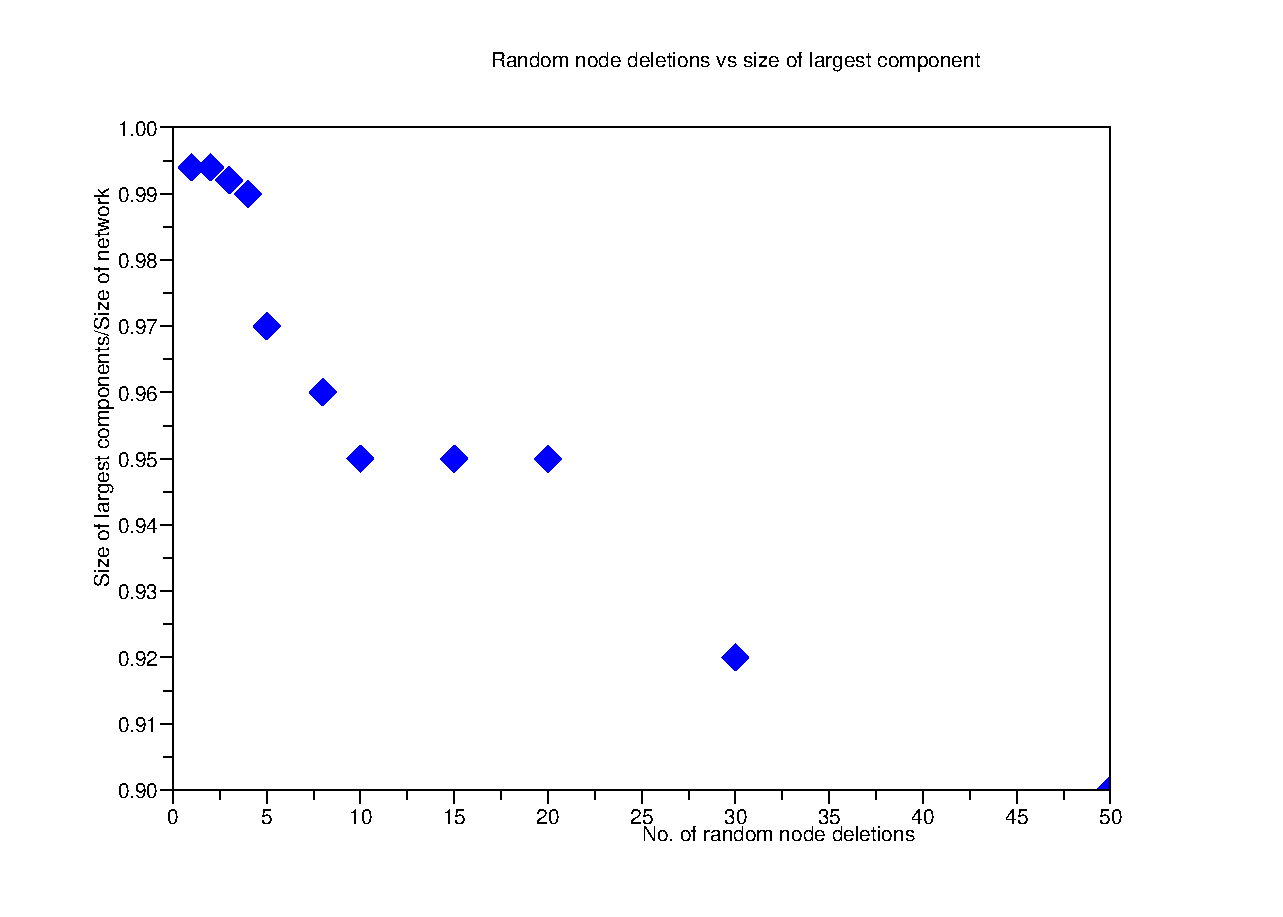
\includegraphics{continental-scc}[htp]% Here is how to import EPS art
\end{center}
\caption{\label{fig:scc}Effect of random node deletions on functional robustness.}
\end{figure*}

%
%\subsubsection{Selection Pressure Estimate}
%Venkatasubramanian et al.~\cite{venkat04} propose the selection pressure variable $\alpha$ that decides the trade-off between efficiency and robustness during the design process of a complex network. In this work, we propose a complementary measure $\beta$ which is an \textit{estimate} of $\alpha$ that might have been used to design a particular network topology.

%\section{Classes of Complex Networks}
%\subsection{Foodwebs}
%\subsection{Supply Chain Networks}
%\subsection{Airline Networks}
%
%\section{Performance Analyses}


%\subsection{Efficiency Analyses}
%\subsection{Robustness Analyses}
%\subsection{Comparison with Random Graphs}
%\subsection{Interesting Design Motifs}

%\section{Related Literature and Discussion}
%There is a lot of recent interest in developing a philosophical understanding of the design of complex networks. %in several domains. %Structural properties of complex networks have been studied extensively, especially following the seminal work by Strogatz, Albert and Barab\`{a}si~\cite{strogatz01, albert02, barabasi03}. 
%Disparate classes of complex networks such as the Internet~\cite{faloutsos99}, WWW~\cite{albert99}, metabolic networks~\cite{guimera07, smart08}, foodwebs~\cite{williams00}, protein interaction networks~\cite{jeong01, guimera04b} and social networks~\cite{newman03} have been analyzed. There are attempts to relate their structural properties such as density, diameter, degree distribution, betweenness distribution, clustering coefficient and modularity, to their performance. 
%
%A large body of literature exists that attempts to characterize complex networks inspired from ideas in statistical physics such as \textit{emergence} and \textit{self-organization}. The most popular model of self-organization is \textit{self-organized criticality} (SOC) proposed by Bak~\cite{bak86}. The essential intuition behind SOC is that systems with a large number of interacting components will ``self-organize'' to a critical point at which occurrence of events follows a power law. Since this behaviour ``emerges'' without the need for tuning parameters, system design has only a secondary role.
%
%Network generation models developed in efforts to explain seemingly universal motifs in complex networks such as power law degree distribution, community structures and small diameters use ideas similar to SOC. Barab\`{a}si and Albert~\cite{barabasi03} propose preferential attachment as the underlying mechanism for the emrgence of power laws in nature and man-made networks. Watts and Strogatz~\cite{watts98} propose a model to generate networks that exhibit ``small-world'' properties with small average path lengths and high clustering coefficients leading to the formation of ``communities''. The Watts-Strogatz model uses a parameter that determines the amount of randomness in the network. Kleinberg~\cite{kleinberg00} provides a theoretical framework for small-world networks by developing exact conditions under which small-worlds occur. Newman~\cite{newman06} reports the existence of community structures in disparate complex networks.
%
%In contrast to the statistical mechanical explanations of phenomema like power laws as emerging due to simple underlying forces like  PA, there are recent efforts which propose that the occurrence of complex phenomena are a result of rigorous design for performance. A network's functional requirements are defined in terms of optimality objectives. The occurrence of interesting motifs is thus the result of trade-offs between objectives. Carlson and Doyle~\cite{carlson99} propose \textit{highly optimized tolerance} (HOT), a mechanism to generate power laws as a result of trade-offs between efficiency and robustness in a network. They also challenge the validity of models such as PA since those models ignore domain dependent trade-offs~\cite{alderson05}. Further, preferential attachment models attempts to characterize networks based solely on degree distribution, which might be inadequate~\cite{willinger09}. For example, analysis of WAN~\cite{guimera04} shows that PA cannot explain the seemingly anomolous betweenness centrality values.

\section{Future Work}
%* What are complex networks: (1) man made (2) natural\\
%
%* Special structural properties -- structure influences function\\
%
%* Efficiency, robustness and cost as three principal dimensions.\\
%
%* In this work, we study: (1) structural properties (2) subject a variety of complex n/ws to graph theoretic analysis (2) wrt eff, rob and cost.\\


%\section{Related Literature}
%Subsection text here.
%
%
%
%\subsection{Efficiency measures}
%* APL\\
%* Diameter\\
%
%\subsection{Robustness measures}
%* SECON measures\\
%* Degree distribution based\\
%* Connectivity based\\
%* Centrality based measures\\
%
%\subsection{Cost measures}
%* Redundancy\\
%* Density\\
%
%\section{Efficiency and Robustness Analyses}
%
%\section{Discussion}


%When commands are referred to in this example file, they are always
%shown with their required arguments, using normal \TeX{} format. In
%this format, \verb+#1+, \verb+#2+, etc. stand for required
%author-supplied arguments to commands. For example, in
%\verb+\section{#1}+ the \verb+#1+ stands for the title text of the
%author's section heading, and in \verb+\title{#1}+ the \verb+#1+
%stands for the title text of the paper.
%
%Line breaks in section headings at all levels can be introduced using
%\textbackslash\textbackslash. A blank input line tells \TeX\ that the
%paragraph has ended. Note that top-level section headings are
%automatically uppercased. If a specific letter or word should appear in
%lowercase instead, you must escape it using \verb+\lowercase{#1}+ as
%in the word ``via'' above.

%\subsection{\label{sec:level2}Second-level heading: Formatting}
%
%This file may be formatted in both the \texttt{preprint} and
%\texttt{twocolumn} styles. \texttt{twocolumn} format may be used to
%mimic final journal output. Either format may be used for submission
%purposes; however, for peer review and production, APS will format the
%article using the \texttt{preprint} class option. Hence, it is
%essential that authors check that their manuscripts format acceptably
%under \texttt{preprint}. Manuscripts submitted to APS that do not
%format correctly under the \texttt{preprint} option may be delayed in
%both the editorial and production processes.
%
%The \texttt{widetext} environment will make the text the width of the
%full page, as on page~\pageref{eq:wideeq}. (Note the use the
%\verb+\pageref{#1}+ to get the page number right automatically.) The
%width-changing commands only take effect in \texttt{twocolumn}
%formatting. It has no effect if \texttt{preprint} formatting is chosen
%instead.
%
%\subsubsection{\label{sec:level3}Third-level heading: References and Footnotes}
%Reference citations in text use the commands \verb+\cite{#1}+ or
%\verb+\onlinecite{#1}+. \verb+#1+ may contain letters and numbers.
%The reference itself is specified by a \verb+\bibitem{#1}+ command
%with the same argument as the \verb+\cite{#1}+ command.
%\verb+\bibitem{#1}+ commands may be crafted by hand or, preferably,
%generated by using Bib\TeX. REV\TeX~4 includes Bib\TeX\ style files
%\verb+apsrev.bst+ and \verb+apsrmp.bst+ appropriate for
%\textit{Physical Review} and \textit{Reviews of Modern Physics},
%respectively. REV\TeX~4 will automatically choose the style
%appropriate for the journal specified in the document class
%options. This sample file demonstrates the basic use of Bib\TeX\
%through the use of \verb+\bibliography+ command which references the
%\verb+assamp.bib+ file. Running Bib\TeX\ (typically \texttt{bibtex
%apssamp}) after the first pass of \LaTeX\ produces the file
%\verb+apssamp.bbl+ which contains the automatically formatted
%\verb+\bibitem+ commands (including extra markup information via
%\verb+\bibinfo+ commands). If not using Bib\TeX, the
%\verb+thebibiliography+ environment should be used instead.
%
%To cite bibliography entries, use the \verb+\cite{#1}+ command. Most
%journal styles will display the corresponding number(s) in square
%brackets: \cite{feyn54,witten2001}. To avoid the square brackets, use
%\verb+\onlinecite{#1}+: Refs.~\onlinecite{feyn54} and
%\onlinecite{witten2001}. REV\TeX\ ``collapses'' lists of
%consecutive reference numbers where possible. We now cite everyone
%together \cite{feyn54,witten2001,epr}, and once again
%(Refs.~\onlinecite{epr,feyn54,witten2001}). Note that the references
%were also sorted into the correct numerical order as well.
%
%When the \verb+prb+ class option is used, the \verb+\cite{#1}+ command
%displays the reference's number as a superscript rather than using
%square brackets. Note that the location of the \verb+\cite{#1}+
%command should be adjusted for the reference style: the superscript
%references in \verb+prb+ style must appear after punctuation;
%otherwise the reference must appear before any punctuation. This
%sample was written for the regular (non-\texttt{prb}) citation style.
%The command \verb+\onlinecite{#1}+ in the \texttt{prb} style also
%displays the reference on the baseline.
%
%Footnotes are produced using the \verb+\footnote{#1}+ command. Most
%APS journal styles put footnotes into the bibliography. REV\TeX~4 does
%this as well, but instead of interleaving the footnotes with the
%references, they are listed at the end of the references\footnote{This
%may be improved in future versions of REV\TeX.}. Because the correct
%numbering of the footnotes must occur after the numbering of the
%references, an extra pass of \LaTeX\ is required in order to get the
%numbering correct.

%\section{Math and Equations}
%Inline math may be typeset using the \verb+$+ delimiters. Bold math
%symbols may be achieved using the \verb+bm+ package and the
%\verb+\bm{#1}+ command it supplies. For instance, a bold $\alpha$ can
%be typeset as \verb+$\bm{\alpha}$+ giving $\bm{\alpha}$. Fraktur and
%Blackboard (or open face or double struck) characters should be
%typeset using the \verb+\mathfrak{#1}+ and \verb+\mathbb{#1}+ commands
%respectively. Both are supplied by the \texttt{amssymb} package. For
%example, \verb+$\mathbb{R}$+ gives $\mathbb{R}$ and
%\verb+$\mathfrak{G}$+ gives $\mathfrak{G}$
%
%In \LaTeX\ there are many different ways to display equations, and a
%few preferred ways are noted below. Displayed math will center by
%default. Use the class option \verb+fleqn+ to flush equations left.
%
%Below we have numbered single-line equations; this is the most common
%type of equation in \textit{Physical Review}:
%\begin{eqnarray}
%\chi_+(p)\alt{\bf [}2|{\bf p}|(|{\bf p}|+p_z){\bf ]}^{-1/2}
%\left(
%\begin{array}{c}
%|{\bf p}|+p_z\\
%px+ip_y
%\end{array}\right)\;,
%\\
%\left\{%
% \openone234567890abc123\alpha\beta\gamma\delta1234556\alpha\beta
% \frac{1\sum^{a}_{b}}{A^2}%
%\right\}%
%\label{eq:one}.
%\end{eqnarray}
%Note the open one in Eq.~(\ref{eq:one}).
%
%Not all numbered equations will fit within a narrow column this
%way. The equation number will move down automatically if it cannot fit
%on the same line with a one-line equation:
%\begin{equation}
%\left\{
% ab12345678abc123456abcdef\alpha\beta\gamma\delta1234556\alpha\beta
% \frac{1\sum^{a}_{b}}{A^2}%
%\right\}.
%\end{equation}
%
%When the \verb+\label{#1}+ command is used [cf. input for
%Eq.~(\ref{eq:one})], the equation can be referred to in text without
%knowing the equation number that \TeX\ will assign to it. Just
%use \verb+\ref{#1}+, where \verb+#1+ is the same name that used in
%the \verb+\label{#1}+ command.
%
%Unnumbered single-line equations can be typeset
%using the \verb+\[+, \verb+\]+ format:
%\[g^+g^+ \rightarrow g^+g^+g^+g^+ \dots ~,~~q^+q^+\rightarrow
%q^+g^+g^+ \dots ~. \]
%
%\subsection{Multiline equations}
%
%Multiline equations are obtained by using the \verb+eqnarray+
%environment.  Use the \verb+\nonumber+ command at the end of each line
%to avoid assigning a number:
%\begin{eqnarray}
%{\cal M}=&&ig_Z^2(4E_1E_2)^{1/2}(l_i^2)^{-1}
%\delta_{\sigma_1,-\sigma_2}
%(g_{\sigma_2}^e)^2\chi_{-\sigma_2}(p_2)\nonumber\\
%&&\times
%[\epsilon_jl_i\epsilon_i]_{\sigma_1}\chi_{\sigma_1}(p_1),
%\end{eqnarray}
%\begin{eqnarray}
%\sum \vert M^{\text{viol}}_g \vert ^2&=&g^{2n-4}_S(Q^2)~N^{n-2}
%        (N^2-1)\nonumber \\
% & &\times \left( \sum_{i<j}\right)
%  \sum_{\text{perm}}
% \frac{1}{S_{12}}
% \frac{1}{S_{12}}
% \sum_\tau c^f_\tau~.
%\end{eqnarray}
%\textbf{Note:} Do not use \verb+\label{#1}+ on a line of a multiline
%equation if \verb+\nonumber+ is also used on that line. Incorrect
%cross-referencing will result. Notice the use \verb+\text{#1}+ for
%using a Roman font within a math environment.
%
%To set a multiline equation without \emph{any} equation
%numbers, use the \verb+\begin{eqnarray*}+,
%\verb+\end{eqnarray*}+ format:
%\begin{eqnarray*}
%\sum \vert M^{\text{viol}}_g \vert ^2&=&g^{2n-4}_S(Q^2)~N^{n-2}
%        (N^2-1)\\
% & &\times \left( \sum_{i<j}\right)
% \left(
%  \sum_{\text{perm}}\frac{1}{S_{12}S_{23}S_{n1}}
% \right)
% \frac{1}{S_{12}}~.
%\end{eqnarray*}
%To obtain numbers not normally produced by the automatic numbering,
%use the \verb+\tag{#1}+ command, where \verb+#1+ is the desired
%equation number. For example, to get an equation number of
%(\ref{eq:mynum}),
%\begin{equation}
%g^+g^+ \rightarrow g^+g^+g^+g^+ \dots ~,~~q^+q^+\rightarrow
%q^+g^+g^+ \dots ~. \tag{2.6$'$}\label{eq:mynum}
%\end{equation}
%
%A few notes on \verb=\tag{#1}=. \verb+\tag{#1}+ requires
%\texttt{amsmath}. The \verb+\tag{#1}+ must come before the
%\verb+\label{#1}+, if any. The numbering set with \verb+\tag{#1}+ is
%\textit{transparent} to the automatic numbering in REV\TeX{};
%therefore, the number must be known ahead of time, and it must be
%manually adjusted if other equations are added. \verb+\tag{#1}+ works
%with both single-line and multiline equations. \verb+\tag{#1}+ should
%only be used in exceptional case - do not use it to number all
%equations in a paper.
%
%Enclosing single-line and multiline equations in
%\verb+\begin{subequations}+ and \verb+\end{subequations}+ will produce
%a set of equations that are ``numbered'' with letters, as shown in
%Eqs.~(\ref{subeq:1}) and (\ref{subeq:2}) below:
%\begin{subequations}
%\label{eq:whole}
%\begin{equation}
%\left\{
% abc123456abcdef\alpha\beta\gamma\delta1234556\alpha\beta
% \frac{1\sum^{a}_{b}}{A^2}
%\right\},\label{subeq:1}
%\end{equation}
%\begin{eqnarray}
%{\cal M}=&&ig_Z^2(4E_1E_2)^{1/2}(l_i^2)^{-1}
%(g_{\sigma_2}^e)^2\chi_{-\sigma_2}(p_2)\nonumber\\
%&&\times
%[\epsilon_i]_{\sigma_1}\chi_{\sigma_1}(p_1).\label{subeq:2}
%\end{eqnarray}
%\end{subequations}
%Putting a \verb+\label{#1}+ command right after the
%\verb+\begin{subequations}+, allows one to
%reference all the equations in a subequations environment. For
%example, the equations in the preceding subequations environment were
%Eqs.~(\ref{eq:whole}).
%
%\subsubsection{Wide equations}
%The equation that follows is set in a wide format, i.e., it spans
%across the full page. The wide format is reserved for long equations
%that cannot be easily broken into four lines or less:
%\begin{widetext}
%\begin{equation}
%{\cal R}^{(\text{d})}=
% g_{\sigma_2}^e
% \left(
%   \frac{[\Gamma^Z(3,21)]_{\sigma_1}}{Q_{12}^2-M_W^2}
%  +\frac{[\Gamma^Z(13,2)]_{\sigma_1}}{Q_{13}^2-M_W^2}
% \right)
% + x_WQ_e
% \left(
%   \frac{[\Gamma^\gamma(3,21)]_{\sigma_1}}{Q_{12}^2-M_W^2}
%  +\frac{[\Gamma^\gamma(13,2)]_{\sigma_1}}{Q_{13}^2-M_W^2}
% \right)\;. \label{eq:wideeq}
%\end{equation}
%\end{widetext}
%This is typed to show the output is in wide format.
%(Since there is no input line between \verb+\equation+ and
%this paragraph, there is no paragraph indent for this paragraph.)
%\section{Cross-referencing}
%REV\TeX{} will automatically number sections, equations, figure
%captions, and tables. In order to reference them in text, use the
%\verb+\label{#1}+ and \verb+\ref{#1}+ commands. To reference a
%particular page, use the \verb+\pageref{#1}+ command.
%
%The \verb+\label{#1}+ should appear in a section heading, within an
%equation, or in a table or figure caption. The \verb+\ref{#1}+ command
%is used in the text where the citation is to be displayed.  Some
%examples: Section~\ref{sec:level1} on page~\pageref{sec:level1},
%Table~\ref{tab:table1}, and Fig.~\ref{fig:epsart}.
%
%\section{Figures and Tables}
%Figures and tables are typically ``floats'' which means that their
%final position is determined by \LaTeX\ while the document is being
%typeset. \LaTeX\ isn't always successful in placing floats
%optimally.
%
%Figures may be inserted by using either the \texttt{graphics} or
%\texttt{graphix} packages. These packages both define the
%\verb+\includegraphics{#1}+ command, but they differ in how optional
%arguments for specifying the orientation, scaling, and translation of the
%figure. Fig.~\ref{fig:epsart} shows a figure that is small enough to
%fit in a single column. It is embedded using the \texttt{figure}
%environment which provides both the caption and the imports the figure
%file.
%\begin{figure}
%\includegraphics{fig_1}% Here is how to import EPS art
%\caption{\label{fig:epsart} A figure caption. The figure captions are
%automatically numbered.}
%\end{figure}
%
%Fig.~\ref{fig:wide} is a figure that is too wide for a single column,
%so instead the \texttt{figure*} environment has been used.
%\begin{figure*}
%\includegraphics{fig_2}% Here is how to import EPS art
%\caption{\label{fig:wide}Use the figure* environment to get a wide
%figure that spans the page in \texttt{twocolumn} formatting.}
%\end{figure*}
%
%The heart of any table is the \texttt{tabular} environment which gives
%the rows of the tables. Each row consists of column entries separated
%by \verb+&+'s and terminates with \textbackslash\textbackslash. The
%required argument for the \texttt{tabular} environment
%specifies how data are displayed in the columns. For instance, entries
%may be centered, left-justified, right-justified, aligned on a decimal
%point. Extra column-spacing may be be specified as well, although
%REV\TeX~4 sets this spacing so that the columns fill the width of the
%table. Horizontal rules are typeset using the \verb+\hline+
%command. The doubled (or Scotch) rules that appear at the top and
%bottom of a table can be achieved enclosing the \texttt{tabular}
%environment within a \texttt{ruledtabular} environment. Rows whose
%columns span multiple columns can be typeset using the
%\verb+\multicolumn{#1}{#2}{#3}+ command (for example, see the first
%row of Table~\ref{tab:table3}).
%
%Tables~\ref{tab:table1}-\ref{tab:table4} show various effects. Tables
%that fit in a narrow column are contained in a \texttt{table}
%environment. Table~\ref{tab:table3} is a wide table set with the
%\texttt{table*} environment. Long tables may need to break across
%pages. The most straightforward way to accomplish this is to specify
%the \verb+[H]+ float placement on the \texttt{table} or
%\texttt{table*} environment. However, the standard \LaTeXe\ package
%\texttt{longtable} will give more control over how tables break and
%will allow headers and footers to be specified for each page of the
%table. A simple example of the use of \texttt{longtable} can be found
%in the file \texttt{summary.tex} that is included with the REV\TeX~4
%distribution.
%
%There are two methods for setting footnotes within a table (these
%footnotes will be displayed directly below the table rather than at
%the bottom of the page or in the bibliography). The easiest
%and preferred method is just to use the \verb+\footnote{#1}+
%command. This will automatically enumerate the footnotes with
%lowercase roman letters. However, it is sometimes necessary to have
%multiple entries in the table share the same footnote. In this case,
%there is no choice but to manually create the footnotes using
%\verb+\footnotemark[#1]+ and \verb+\footnotetext[#1]{#2}+.
%\texttt{\#1} is a numeric value. Each time the same value for
%\texttt{\#1} is used, the same mark is produced in the table. The
%\verb+\footnotetext[#1]{#2}+ commands are placed after the \texttt{tabular}
%environment. Examine the \LaTeX\ source and output for
%Tables~\ref{tab:table1} and \ref{tab:table2} for examples.
%
%\begin{table}
%\caption{\label{tab:table1}This is a narrow table which fits into a
%narrow column when using \texttt{twocolumn} formatting. Note that
%REV\TeX~4 adjusts the intercolumn spacing so that the table fills the
%entire width of the column. Table captions are numbered
%automatically. This table illustrates left-aligned, centered, and
%right-aligned columns.  }
%\begin{ruledtabular}
%\begin{tabular}{lcr}
%Left\footnote{Note a.}&Centered\footnote{Note b.}&Right\\
%\hline
%1 & 2 & 3\\
%10 & 20 & 30\\
%100 & 200 & 300\\
%\end{tabular}
%\end{ruledtabular}
%\end{table}
%
%\begin{table}
%\caption{\label{tab:table2}A table with more columns still fits
%properly in a column. Note that several entries share the same
%footnote. Inspect the \LaTeX\ input for this table to see
%exactly how it is done.}
%\begin{ruledtabular}
%\begin{tabular}{cccccccc}
% &$r_c$ (\AA)&$r_0$ (\AA)&$\kappa r_0$&
% &$r_c$ (\AA) &$r_0$ (\AA)&$\kappa r_0$\\
%\hline
%Cu& 0.800 & 14.10 & 2.550 &Sn\footnotemark[1]
%& 0.680 & 1.870 & 3.700 \\
%Ag& 0.990 & 15.90 & 2.710 &Pb\footnotemark[2]
%& 0.450 & 1.930 & 3.760 \\
%Au& 1.150 & 15.90 & 2.710 &Ca\footnotemark[3]
%& 0.750 & 2.170 & 3.560 \\
%Mg& 0.490 & 17.60 & 3.200 &Sr\footnotemark[4]
%& 0.900 & 2.370 & 3.720 \\
%Zn& 0.300 & 15.20 & 2.970 &Li\footnotemark[2]
%& 0.380 & 1.730 & 2.830 \\
%Cd& 0.530 & 17.10 & 3.160 &Na\footnotemark[5]
%& 0.760 & 2.110 & 3.120 \\
%Hg& 0.550 & 17.80 & 3.220 &K\footnotemark[5]
%&  1.120 & 2.620 & 3.480 \\
%Al& 0.230 & 15.80 & 3.240 &Rb\footnotemark[3]
%& 1.330 & 2.800 & 3.590 \\
%Ga& 0.310 & 16.70 & 3.330 &Cs\footnotemark[4]
%& 1.420 & 3.030 & 3.740 \\
%In& 0.460 & 18.40 & 3.500 &Ba\footnotemark[5]
%& 0.960 & 2.460 & 3.780 \\
%Tl& 0.480 & 18.90 & 3.550 & & & & \\
%\end{tabular}
%\end{ruledtabular}
%\footnotetext[1]{Here's the first, from Ref.~\onlinecite{feyn54}.}
%\footnotetext[2]{Here's the second.}
%\footnotetext[3]{Here's the third.}
%\footnotetext[4]{Here's the fourth.}
%\footnotetext[5]{And etc.}
%\end{table}
%

%
%\begin{table}
%\caption{\label{tab:table4}Numbers in columns Three--Five have been
%aligned by using the ``d'' column specifier (requires the
%\texttt{dcolumn} package). Non-numeric entries (those entries without
%a ``.'') in a ``d'' column are aligned on the decimal point. Use the
%``D'' specifier for more complex layouts. }
%\begin{ruledtabular}
%\begin{tabular}{ccddd}
%One&Two&\mbox{Three}&\mbox{Four}&\mbox{Five}\\
%\hline
%one&two&\mbox{three}&\mbox{four}&\mbox{five}\\
%He&2& 2.77234 & 45672. & 0.69 \\
%C\footnote{Some tables require footnotes.}
%  &C\footnote{Some tables need more than one footnote.}
%  & 12537.64 & 37.66345 & 86.37 \\
%\end{tabular}
%\end{ruledtabular}
%\end{table}
%
%\textit{Physical Review} style requires that the initial citation of
%figures or tables be in numerical order in text, so don't cite
%Fig.~\ref{fig:wide} until Fig.~\ref{fig:epsart} has been cited.
%
%\begin{acknowledgments}
%We wish to acknowledge the support of the author community in using
%REV\TeX{}, offering suggestions and encouragement, testing new versions,
%\dots.
%\end{acknowledgments}
%
%\appendix
%
%\section{Appendixes}
%
%To start the appendixes, use the \verb+\appendix+ command.
%This signals that all following section commands refer to appendixes
%instead of regular sections. Therefore, the \verb+\appendix+ command
%should be used only once---to setup the section commands to act as
%appendixes. Thereafter normal section commands are used. The heading
%for a section can be left empty. For example,
%\begin{verbatim}
%\appendix
%\section{}
%\end{verbatim}
%will produce an appendix heading that says ``APPENDIX A'' and
%\begin{verbatim}
%\appendix
%\section{Background}
%\end{verbatim}
%will produce an appendix heading that says ``APPENDIX A: BACKGROUND''
%(note that the colon is set automatically).
%
%If there is only one appendix, then the letter ``A'' should not
%appear. This is suppressed by using the star version of the appendix
%command (\verb+\appendix*+ in the place of \verb+\appendix+).
%
%\section{A little more on appendixes}
%
%Observe that this appendix was started by using
%\begin{verbatim}
%\section{A little more on appendixes}
%\end{verbatim}
%
%Note the equation number in an appendix:
%\begin{equation}
%E=mc^2.
%\end{equation}
%
%\subsection{\label{app:subsec}A subsection in an appendix}
%
%You can use a subsection or subsubsection in an appendix. Note the
%numbering: we are now in Appendix \ref{app:subsec}.
%
%Note the equation numbers in this appendix, produced with the
%subequations environment:
%\begin{subequations}
%\begin{eqnarray}
%E&=&mc, \label{appa}
%\\
%E&=&mc^2, \label{appb}
%\\
%E&\agt& mc^3. \label{appc}
%\end{eqnarray}
%\end{subequations}
%They turn out to be Eqs.~(\ref{appa}), (\ref{appb}), and (\ref{appc}).
%\newpage %Just because of unusual number of tables stacked at end

%\bibliography{apssamp}% Produces the bibliography via BibTeX.

\section{Conclusion}
The conclusion goes here.

\section*{Acknowledgment}
The authors would like to thank...
\begin{thebibliography}{50}

\bibitem{stats2009}
Source: Bureau of Transportation Statistics, T-100 Market

\bibitem{button99}
K. J. Button. \textit{An Assessment of the Capacity and Congestion Levels at European Airports}. Journal of Air Transport Management, 1999.

\bibitem{brueckner05}
J. A. Brueckner. \textit{Internalization of airport congestion: A network analysis}. International Journal of Industrial Organization, 2005.

\bibitem{morrison07}
S. A. Morrison and C. Winston. \textit{Another look at airport congestion pricing}. American Economic Review, 2007.

\bibitem{colizza06}
V. Colizza, A. Barrat�, M. Barth\'{e}lemy and A. Vespignani. \textit{The role of the airline transportation network in the prediction and predictability of global epidemics}. Proc. Natl. Acad. Sci. USA, Vol. 103, pp. 2015�2020.

\bibitem{guimera05}
R. Guimer\`{a}, S. Mossa, A. Turtschi and L. A. N. Amaral. \textit{The worldwide air transportation network: Anomalous centrality, community structure, and cities' global roles}. Proceedings of the National Academy of Sciences, 2005.

\bibitem{brueckner01}
J. A. Brueckner and Y. Zhang. \textit{A Model of Scheduling in Airline Networks: How a Hub-and-Spoke System Affects Flight Frequency, Fares and Welfare}. Journal of Transport Economics and Policy, Vol. 35, No. 2 (May, 2001), pp. 195-222.

\bibitem{burghouwt02}
G. Burghouwt and J. Hakfoort. \textit{The evolution of the European aviation network, 1990�1998}. Journal of Air Transport Management, 2001.

\bibitem{button02}
K. Button. \textit{Debunking some common myths about airport hubs}. Journal of Air Transport Management, 2002.

\bibitem{berry06}
S. Berry, M. Carnall and P. T. Spiller. Airline hubs: costs, markups and the implications of customer heterogeneity. Competition Policy and Antitrust, 2006

\bibitem{alderighi07}
M. Alderighi, A. Cento, P. Nijkamp and P. Rietveld. \textit{Network competition: the coexistence of hub-and-spoke and point-to-point systems}. Journal of Air Transport Management, 2005.

\bibitem{adler06}
N. Adler and K. Smilowitz. \textit{Hub-and-spoke network alliances and mergers: Price-location competition in the airline industry}. Transportation Research Part B, 2007.

\bibitem{alumur08}
S. Alumur and B. Y. Kara. \textit{Network hub location problems: The state of the art}. European Journal of Operational Research, 2008.

\bibitem{mcafee06}
R. P. McAfee, V. Te Velde. \textit{Dynamic pricing in the airline industry}. Economics and Information Systems, 2006.

\bibitem{forbes08}
S. J. Forbes. \textit{The effect of air traffic delays on airline prices}. International Journal of Industrial Organization, 2008.

\bibitem{guimera04}
R. Guimera and L. A. N. Amaral. \textit{Modeling the worldwide airport network}.  The European Physical Journal B, 2004.

\bibitem{barrat04}
A. Barrat, M. Barth\'{e}lemy, R. Pastor-Satorras and A. Vespignani. \textit{The architecture of complex weighted networks}. Proceedings of the National Academy of Sciences, 2004.

\bibitem{newman03}
M. E. J. Newman and M. Girvan. \textit{Mixing patterns and community structure in networks}. Proceedings on a Workshop on Statistics on Networks, 2007.

\bibitem{barthelemy04}
M. Barth\'{e}lemy, A. Barrat, R. Pastor-Satorras and A. Vespignani. \textit{Characterization and modeling of weighted networks}. Physica A: Statistical Mechanics and Its Applications, 2005.

\bibitem{li04}
W. Li and X. Cai. \textit{Statistical analysis of airport network of China}. Phys Rev E, 2004.

\bibitem{bagler08}
G. Bagler. \textit{Analysis of the Airport Network of India as a complex weighted network}. Physica A: Statistical Mechanics and its Applications, 2008.

\bibitem{guida06}
M. Guida and F. Maria. \textit{Topology of the Italian airport network: A scale-free small-world network with a fractal structure?}. Chaos, Solitons and Fractals, 2007.

\bibitem{sienkiewicz05}
J. Sienkiewicz and J. A. Holyst. \textit{Statistical analysis of 22 public transport networks in Poland}. Physical review. E, Statistical, nonlinear, and soft matter physics, 2005.

\bibitem{haversine}
http://en.wikipedia.org/wiki/Haversine_formula

\bibitem{venkat04}
V. Venkatasubramanian, S. Katare, P. R. Patkar and F. Mu. \textit{Spontaneous emergence of complex optimal networks through evolutionary adaptation}. Computers and Chemical Engineering, 2004.

\bibitem{albert02}
R. Albert and A.-L. Barab\'{a}si. \textit{Statistical mechanics of complex networks}. Review of Modern Physics, 74, pp. 47-97, 2002.

\bibitem{barabasi}
A.-L. Barab\'{a}si. \textit{Scale-Free Networks}. Scientific American, 288, pp. 60-69, May 2003.

\bibitem{strogatz}
S.H. Strogatz. \textit{Exploring complex networks}. Nature, Vol. 410, Issue 6825, pp. 268-276, 2001.

\bibitem{barabasi99}
R. Albert, H. Jeong and A.-L. Barab\'{a}si. \textit{Diameter of the world-wide web}. Nature, Vol. 401, Issue 6749, pp. 130-131, 1999.

\bibitem{watts}
D.J. Watts and S.H. Strogatz. \textit{Collective dynamics of 'small-world' networks}. Nature, Vol. 393, Issue 6684, pp. 440-442,v 1998.

\bibitem{kleinberg}
J.M. Kleinberg. \textit{Navigation in a small world}. Nature, Vol. 406, Issue 6798, pp. 845, 2000.

\bibitem{newman}
M.E.J Newman. \textit{Modularity and community structure in networks}. In proc. National Academy of Sciences, Vol. 103, No. 23, pp. 8577-8582, 2006.

\bibitem{guimera07}
R. Guimera, M. Sales-Pardo and L.A.N. Amaral. A network-based method for target selection in metabolic networks. Bioinformatics 23, 1616-1622 (2007).

\bibitem{amaral08}
Smart, AG, Amaral, LAN, & Ottino, JM. Cascading failure and robustness in metabolic networks. Proc. Natl. Acad. Sci. U. S. A. 105, 13223-13228 (2008).

\end{thebibliography}

\end{document}
%
% ****** End of file apssamp.tex ******
